\documentclass{beamer}

\usepackage{polski}
\usepackage[utf8]{inputenc}
\usepackage{color}
\usepackage{amsfonts}	% Real

\usepackage{booktabs} % eleganckie tabelki


\usetheme{boxes}      % Wybór tematu wyglądu, gdy chcemy inny
%\usecolortheme{rose}   % Wybór tematu kolorystycznego, j.w.

%Konfiguracja dla pakietu hyperref:
\hypersetup{
  unicode=true,           % włączenie wyświetlania pliterek w zakładkach
%  pdfpagemode=FullScreen, % włączenie trybu pełnoekranowanego
  pdfsubject=Graph Neural Networks,      % temat prezentacji
  pdfkeywords={gnn, graph neural network, graph, classification} % slowa kluczowe
}

%% Dane do strony tytułowej
\author{Aleksy Barcz\\mgr inż. Zbigniew Szymański\\ dr inż. Stanisław Jankowski}
\title{Implementation aspects of\\Graph Neural Networks}
\date{\today}
\institute{Warsaw University of Technology}

\setbeamercovered{transparent}

\begin{document}
\frame{\titlepage}

\begin{frame}
\frametitle{What is a Graph Neural Network?}
\begin{itemize}
	\item Scarselli et al., 2009
	\item Classifier of graphs
	\item Most graph types, including nonpositional and cyclic
	\item Node/Graph classification
	\item Based on simple FNN units
\end{itemize}
\end{frame}

\begin{frame}
\frametitle{Encoding network}
\begin{center}
	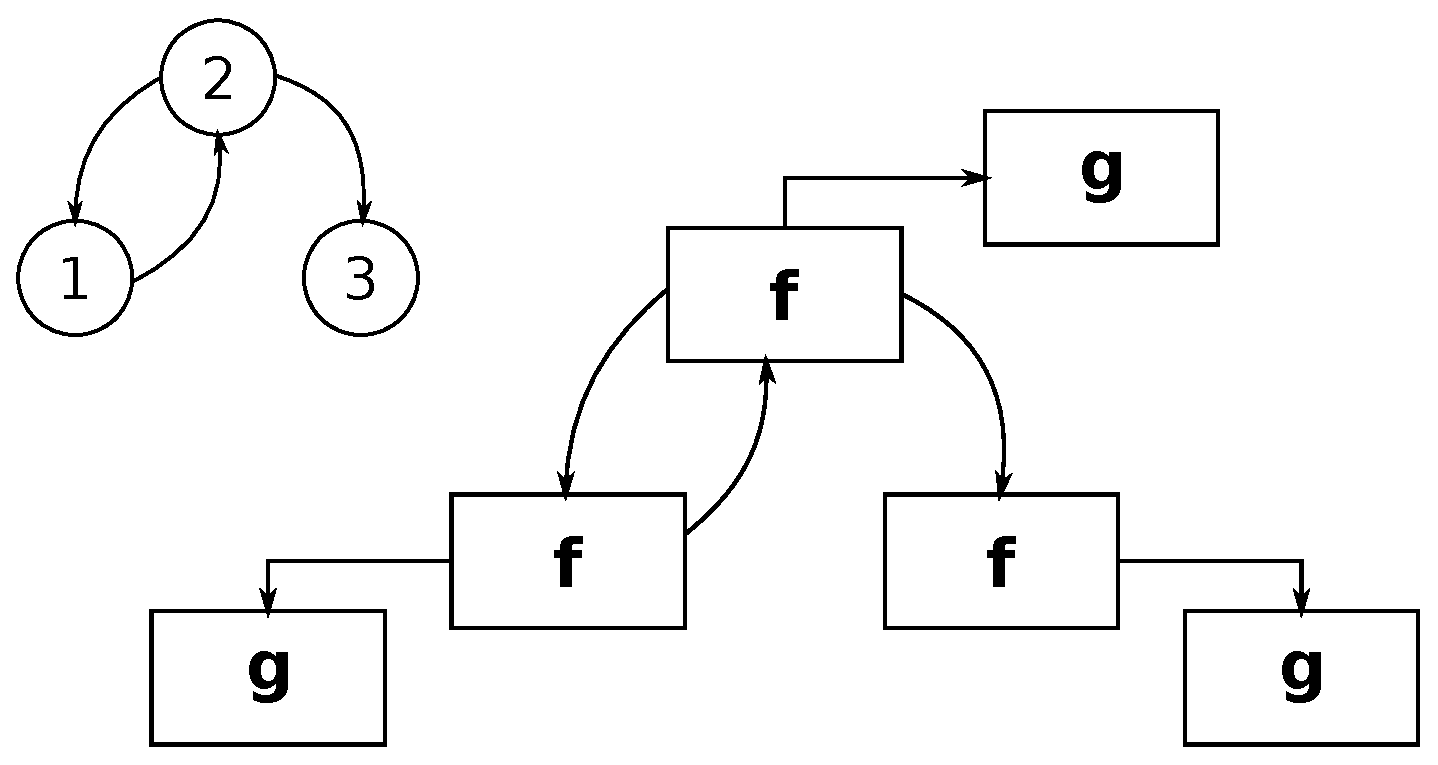
\includegraphics[scale=0.4]{img/encodinginc}
\end{center}
\begin{itemize}
	\item Building node representation: $x_n = f(...)$
	\item Node classification: $o_n = g(x_n)$
	\item All instances of $f_w$ share weights
	\item All instances of $g_w$ share weights
\end{itemize}
\end{frame}

\begin{frame}
\frametitle{Forward - building representation}
\begin{columns}
	\begin{column}{0.66\textwidth}
		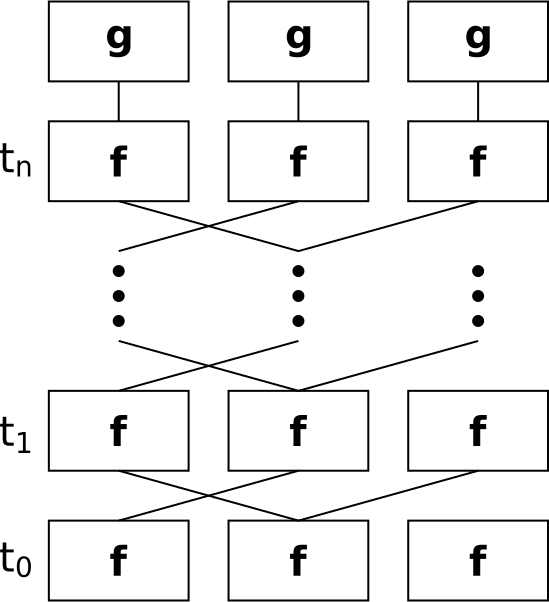
\includegraphics[scale=0.4]{img/forward}
	\end{column}
	\begin{column}{0.34\textwidth}
		\begin{itemize}
			\item unfolding
		\end{itemize}
	\end{column}
\end{columns}
\end{frame}

\begin{frame}
\frametitle{Backward - backpropagation}
\begin{columns}
	\begin{column}{0.66\textwidth}
		\includegraphics[scale=0.4]{img/backward}
	\end{column}
	\begin{column}{0.34\textwidth}
		\begin{itemize}
			\item BPTT
			\item Almeida-Pineda
		\end{itemize}
	\end{column}
\end{columns}
\end{frame}

\begin{frame}
\frametitle{How do we know $F_w$ will reach fixed point?}
\begin{itemize}
	\item contraction map (Banach theorem)
	\item penalty imposed on $F_w$ weights when the contraction is lost
\end{itemize}
\end{frame}

\begin{frame}
\frametitle{How strong should the penalty be?}
\begin{center}
	\includegraphics[scale=0.065]{img/rmse1_clipped}
\end{center}
\begin{itemize}
	\item $contractionConstant \in [1.2, 0.9, 0.6]$
	\item boundary value depends on dataset
\end{itemize}
\end{frame}

\begin{frame}
\frametitle{Results - 5fold crossvalidation, subgraph matching}
\setlength{\tabcolsep}{2pt}
\begin{table}[h!]
	\begin{center}
	\begin{tabular}{llll}
	\toprule
	& accuracy & precision & recall \\
	\midrule
	GNN - tr &	91\% &  87\%&  97\% \\
	GNN - tst &	91\% &  86\% &  97\% \\
	\bottomrule
	\end{tabular}
	\caption{Mean values - GNN}
	\end{center}
\end{table}

\begin{table}[h!]
	\begin{center}
	\begin{tabular}{llll}
	\toprule
	& accuracy & precision & recall \\
	\midrule
	FNN - tr &	71\% &  65\% & 93\% \\
	FNN - tst &	71\% &  64\% &  93\% \\
	\bottomrule
	\end{tabular}
	\caption{Mean values - FNN}
	\end{center}
\end{table}
\end{frame}

\end{document}
